\documentclass{hopescience}
\usepackage{hopescience}

\title{函数拟合实验报告}
\author{高宽 2252708}
\date{\today}

\begin{document}
\maketitle
\tableofcontents

\vspace{5em}
\section{代码作用}
使用一个双层ReLU网络拟合一个基本初等函数,从而验证通用近似定理。其中,网络搭建只使用numpy,利用numpy实现自动梯度。这次任务非常简单,读了文档的原理,看看代码,很容易完成。在进行实验的过程中,我还深入推理了softmax函数的反向传播公式,对反向获得了更加深刻的理解。

\section{函数定义}
待拟合的目标函数为:
\begin{equation}
    f(x) = \frac{\sin(x) + \cos(x)}{\exp(x)} - x^4
\end{equation}

\section{数据采集}
使用numpy即可快速生成数据。代码如下:
\begin{minted}{python}
x = np.linspace(-np.pi, np.pi, 1000).reshape(-1, 1)
y = (np.sin(x) + np.cos(x)) / np.exp(x) - x ** 4
\end{minted}

\section{模型描述}
本实验采用双层ReLU网络,输入和输出层维度均为1,隐藏层维度可以自定义。\cref{fig:network}为网络架构图。

\begin{figure}[H]
    \centering
    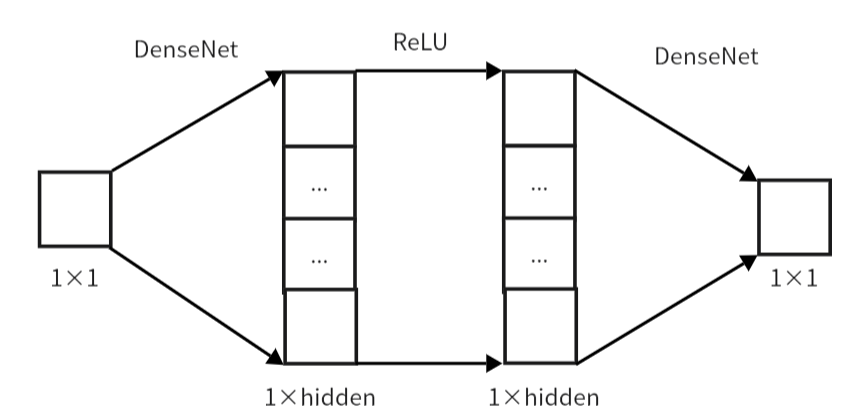
\includegraphics[width=0.5\textwidth]{images/netarch.png}
    \caption{网络架构图}
    \label{fig:network}
\end{figure}

实现该模型的过程中,需要自行定义正向传播和反向传播的计算函数。下面给出其推导的原理。

对于神经网络中的任意一次计算或变形操作,均有输入和输出。设函数为f,输入为x,输出为h,待求偏导的变量为w。w为向量或矩阵。在一次前向传播后,为了更新参数,我们需要求出损失函数对参数的梯度: $ \frac{\phi L}{\phi w} $,其形状于w相同。根据矩阵分析,有:
$$ \frac{\phi L}{\phi w} = \frac{\phi L}{\phi h} \dot \frac{\phi h}{\phi w} $$
这里的乘法是不一定矩阵乘法。在计算中,我们会根据具体情况,在确保遵守链式法则的前提下,使用尽可能简洁地方法将$\frac{\phi L}{\phi h}$与$\frac{\phi h}{\phi w}$结合算出$\frac{\phi L}{\phi w}$算出。$\frac{\phi L}{\phi h}$对于中间层来说,可以直接从后一层的反向传播中获得,对于最后一层来说,可以直接根据求导法则和损失函数,利用预测值与真实值求出,因此$\frac{\phi L}{\phi h}$,总是可以当作反向传播函数的参数传入。$\frac{\phi L}{\phi w}$则可以根据矩阵分析中学过的求导法则求出。综上,在一次训练中,我们总是可以通过反向传播计算出损失函函数对任意参数的梯度! 以乘法计算为例,其代码为:
\begin{minted}{python}
class Mul():
def __init__(self):
    self.mem = {}

def forward(self, inp, w):
    # inp.shape: (N, num_features)
    # w.shape: (in_dim, out_dim)
    # outp.shape: (N, out_dim)
    self.mem['inp'] = inp
    self.mem['w'] = w
    # print(inp.shape, w.shape)
    outp = inp @ w
    return outp

def backward(self, grad_outp):
    # grad_outp.shape: (N, out_dim)
    # grad_inp.shape: (N, num_features)
    # grad_w.shape: (in_dim, out_dim)
    grad_inp = np.matmul(grad_outp, self.mem['w'].T)
    grad_w = np.matmul(self.mem['inp'].T, grad_outp)
    return grad_inp, grad_w
\end{minted}
ReLU操作的正反向传播与之类似。

我们利用上述原理即可实现基于numpy的自动梯度。

\section{拟合效果}
训练时使用MES作为拟合的损失函数。由于待拟合的函数比较简单,样本点也比较少,所以训练时不分批次,每一轮都直接拿整个数据集做训练(也可以认为批大小为1000)。经过多次实验,我们选取隐藏层维度为400、学习率为0.0000005、训练30000轮的经验值。\cref{fig:result}训练所得结果。

\begin{figure}[H]
    \centering
    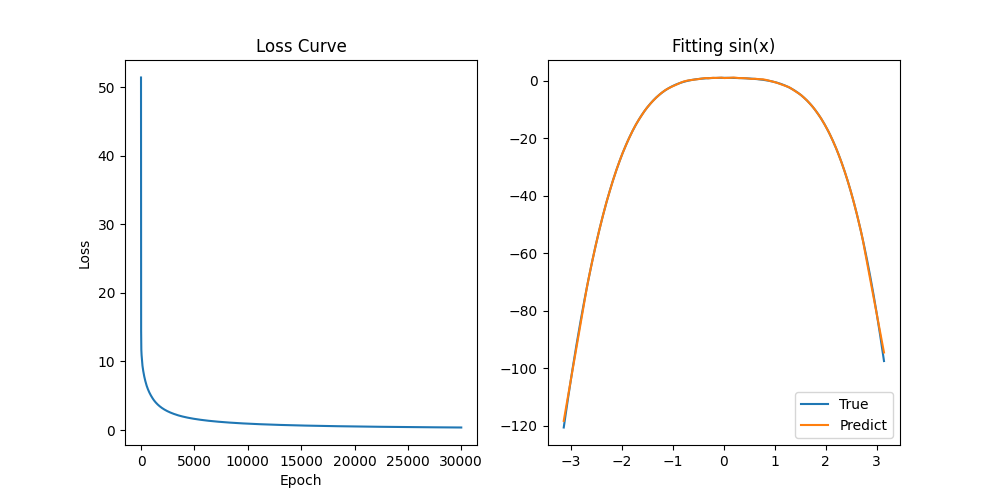
\includegraphics[scaler=0.5]{images/result.png}
    \caption{拟合结果}
    \label{fig:result}
\end{figure}

% printbibliography[heading=bibintoc,title={参考文献}]

\end{document}